\documentclass[11pt]{article}
\usepackage[utf8]{inputenc}
\usepackage{amsmath, amssymb, physics}
\usepackage{geometry}
\usepackage{tcolorbox}
\usepackage{tikz}
\usetikzlibrary{shapes.geometric, arrows.meta, positioning, fit, backgrounds}
\usepackage{hyperref}

\geometry{letterpaper, margin=1in}

\title{\textbf{Theoretical Foundations of UCC: \\ A Multi-Level Compiler for Universal Quantum Computing}}
\author{\textit{A Conceptual Guide for Quantum Practitioners}}
\date{}

\begin{document}

\maketitle

\begin{abstract}
\noindent \textbf{UCC} (the Universal Compiler Collection) is a high-performance quantum circuit compiler and execution engine that fundamentally decouples the geometric structure of a quantum state from its probabilistic execution. Traditional generalized stabilizer simulators dynamically update large Boolean tableaus at runtime, creating severe performance bottlenecks. UCC shifts this heavy mathematics entirely into a multi-level Ahead-Of-Time (AOT) compiler. By natively embracing universal fault-tolerant operations—including non-Clifford rotations, stochastic noise, and projective measurements—the runtime Virtual Machine (VM) is reduced to evaluating $\mathcal{O}(1)$ bitwise operations and managing a dense array of continuous amplitudes. This document defines the theoretical boundaries of the UCC framework, its pure-state mathematical formulation, the algebraic optimization of its intermediate representations, and the concrete instructions that drive its VM.
\end{abstract}

\vspace{0.5cm}

\section{The Core Insight: Topological Determinism and Pure States}

Let a quantum circuit be a sequence of operations $C = (O_0, O_1, \dots, O_{N-1})$, where each $O_t$ is drawn from a strictly defined set of supported operations. In the generalized stabilizer formalism, the quantum state at any step $t$ is anchored by a reference stabilizer-destabilizer tableau $T_t = (\mathcal{S}_t, \mathcal{D}_t)$. The $n$ destabilizers $d_{t,\alpha}$ act as ladder operators to create a full orthogonal basis for the Hilbert space.

\textbf{What is the ``Geometry''?} The geometry of the simulation is defined as the exact sequence of Boolean matrices representing the tableaus $T_0 \to T_1 \to \dots \to T_{N-1}$.

UCC is built on the mathematical property of \textbf{Topological Determinism}: in quantum circuits devoid of classically-controlled Clifford gates, the sequence of tableaus $\{T_t\}$ depends \textit{strictly} on the Clifford gates and the Boolean structure of measurement updates. Probabilistic Pauli noise merely flips scalar $\pm 1$ signs. Non-Clifford gates expand the state into orthogonal superpositions. Random measurement outcomes only flip the signs of newly formed generators. None of these stochastic or branching operations warp the underlying Boolean matrix grid. Therefore, the geometric evolution of the frame is entirely deterministic and can be computed Ahead-Of-Time (AOT).

Because stochastic events (measurements, Pauli noise) are resolved classically per Monte Carlo shot, the underlying complex array managed by the UCC Virtual Machine always tracks a \textit{pure state} superposition over the shifted Pauli frame:
\begin{equation}
    \ket{\phi} = \sum_{\alpha \in \text{span}(V)} v_\alpha d_\alpha \ket{\psi_S}
\end{equation}
where $V$ is the active $k$-dimensional GF(2) spatial shift basis tracked by the compiler. By keeping the state pure within individual shots, memory complexity is strictly bounded to $\mathcal{O}(2^k)$, breaking the $\mathcal{O}(2^{2k})$ quadratic memory bottleneck of analytic density matrix simulators.

\section{System Architecture}

To exploit Topological Determinism, UCC operates as a strict four-stage compiler pipeline. The heavy $\mathcal{O}(n^2)$ geometric tracking is confined to the AOT stages, leaving a perfectly flat, highly vectorized instruction stream for the VM.

\begin{figure}[h!]
\centering
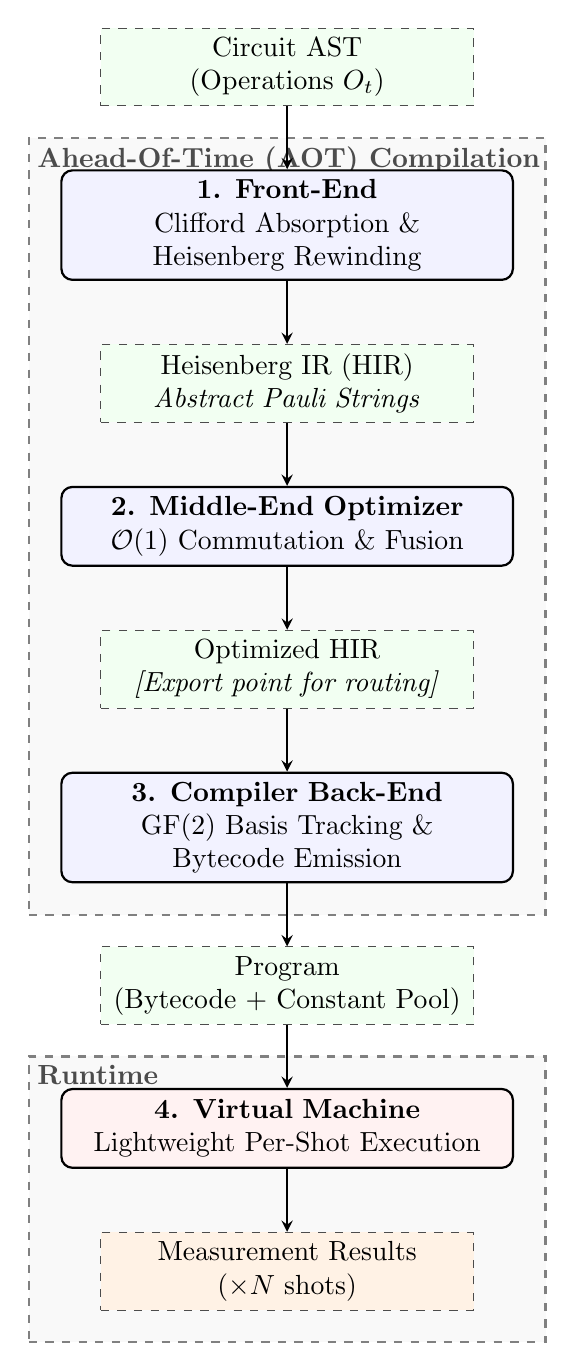
\begin{tikzpicture}[
    node distance=1.2cm and 2cm,
    box/.style={rectangle, draw=black, thick, fill=blue!5, text width=5.5cm, align=center, minimum height=1cm, rounded corners},
    io/.style={rectangle, draw=black!70, dashed, fill=green!5, text width=4.5cm, align=center, minimum height=0.8cm},
    arrow/.style={->, >=stealth, thick}
]

% Nodes
\node[io] (ast) {Circuit AST\\(Operations $O_t$)};
\node[box, below=0.8cm of ast] (frontend) {\textbf{1. Front-End}\\Clifford Absorption \&\\Heisenberg Rewinding};
\node[io, below=0.8cm of frontend] (hir) {Heisenberg IR (HIR)\\ \textit{Abstract Pauli Strings}};
\node[box, below=0.8cm of hir] (middle) {\textbf{2. Middle-End Optimizer}\\$\mathcal{O}(1)$ Commutation \& Fusion};
\node[io, below=0.8cm of middle] (opthir) {Optimized HIR\\ \textit{[Export point for routing]}};
\node[box, below=0.8cm of opthir] (backend) {\textbf{3. Compiler Back-End}\\GF(2) Basis Tracking \&\\Bytecode Emission};
\node[io, below=0.8cm of backend] (program) {Program\\(Bytecode + Constant Pool)};
\node[box, fill=red!5, below=0.8cm of program] (vm) {\textbf{4. Virtual Machine}\\Lightweight Per-Shot Execution};
\node[io, fill=orange!10, below=0.8cm of vm] (results) {Measurement Results\\($\times N$ shots)};

% Bounding box for AOT Compiler
\begin{scope}[on background layer]
    \node[draw=black!50, dashed, thick, fill=gray!5, fit=(frontend) (hir) (middle) (opthir) (backend), inner sep=0.4cm, label={[anchor=north west, font=\bfseries, color=black!70]north west:Ahead-Of-Time (AOT) Compilation}] (aot) {};
\end{scope}

% Bounding box for Runtime
\begin{scope}[on background layer]
    \node[draw=black!50, dashed, thick, fill=gray!5, fit=(vm) (results), inner sep=0.4cm, label={[anchor=north west, font=\bfseries, color=black!70]north west:Runtime}] (runtime) {};
\end{scope}

% Arrows
\draw[arrow] (ast) -- (frontend);
\draw[arrow] (frontend) -- (hir);
\draw[arrow] (hir) -- (middle);
\draw[arrow] (middle) -- (opthir);
\draw[arrow] (opthir) -- (backend);
\draw[arrow] (backend) -- (program);
\draw[arrow] (program) -- (vm);
\draw[arrow] (vm) -- (results);

\end{tikzpicture}
\caption{The UCC Multi-Level Architecture.}
\label{fig:architecture}
\end{figure}

\section{Stage 1: The Front-End (Trace Generation)}

The Front-End mathematically maintains the deterministic reference tableau $T_t$. Its core responsibility is to intercept quantum operations, abstract away their geometric tracking, and emit the \textbf{Heisenberg IR (HIR)}. It does \textbf{not} emit VM opcodes.

\subsection{Clifford Absorption}
If $O_t$ is a pure Clifford gate (e.g., $H, \text{CNOT}, S$), the compiler applies it to advance the reference frame: $T_{t+1} = O_t T_t O_t^\dagger$. Because this frame advancement is entirely deterministic, Clifford gates are completely absorbed. They vanish from the representation entirely and do not produce an HIR node.

\subsection{Heisenberg Rewinding and the Parity Masks}
If $O_t$ is a non-Clifford gate, measurement, or Pauli noise channel, the Front-End rewinds its physical Pauli operator $P_t$ backward through the geometric frame to $t=0$:
\begin{equation}
    P_{t \to 0} = U_{0 \to t}^\dagger P_t U_{0 \to t} \propto \prod_{i=1}^n (s_{0,i})^{c^Z_i} (d_{0,i})^{c^X_i}
\end{equation}
where $U_{0 \to t}$ is the cumulative unitary evolution of all deterministic geometric updates up to time $t$. This exact decomposition yields two vital binary vectors, known as the \textbf{Noise Parity Masks}:
\begin{itemize}
    \item \textbf{\texttt{stab\_mask}} ($c^Z \in \mathbb{F}_2^n$): Identifies which $t=0$ stabilizers compose the rewound operator.
    \item \textbf{\texttt{destab\_mask}} ($c^X \in \mathbb{F}_2^n$): Identifies which $t=0$ destabilizers compose the rewound operator.
\end{itemize}
These masks tell the downstream pipeline exactly how this operation interacts with the static reference frame, encoding both topological shifts and physical noise vulnerabilities.

\begin{tcolorbox}[colback=blue!5,colframe=blue!40!black,title=Dominant Term Factoring]
To simulate universal operations like a $T$-gate, UCC expands them via a Linear Combination of Unitaries (LCU). Naively branching these terms causes floating-point instability.

UCC enforces \textbf{Dominant Term Factoring}. Every non-Clifford gate is refactored into the form $I + c P$, where $I$ is the identity path, $P$ is a Pauli operator, and $c \in \mathbb{C}$ is a relative complex weight. By factoring out the dominant $I$ term, the base path of the quantum state requires \textbf{zero mathematical operations and zero memory writes} at runtime. The extracted global scalar is accumulated deterministically by the compiler into a \texttt{global\_weight} accumulator, enabling the Optimized HIR to be exported directly to physical hardware routers (such as Pauli-Based Computation / tqec) without amplitude distortion.
\end{tcolorbox}

\textbf{Multi-Pauli Measurements.} Because the Front-End rewinds any observable into the $t=0$ frame, complex multi-qubit measurements (such as $M_{X \otimes X \otimes Z}$) are natively supported. A multi-Pauli measurement simply yields a single \texttt{HeisenbergOp} with multiple bits set in its Pauli masks. The Middle-End and Back-End process a weight-10 parity check with the exact same $\mathcal{O}(1)$ bitwise mask complexity as a single-qubit measurement.

\subsection{The Heisenberg IR (HIR)}
The output of the Front-End is the HIR: a flat, algebraically independent list of abstract Pauli string operations (\texttt{HeisenbergOp}). The HIR contains absolutely no VM-specific memory routing or execution semantics. Each operation is defined strictly by its \texttt{OpType}, its two Parity Masks, and a specific data payload:

\begin{itemize}
    \item \textbf{\texttt{T\_GATE} / \texttt{T\_DAG\_GATE}:} Represents the fast-path $T$ and $T^\dagger$ gates. \textit{Payload:} Empty. (The relative weights $\mp i \tan(\pi/8)$ are mathematically implicit).
    \item \textbf{\texttt{GATE}:} A generic non-Clifford LCU operation (e.g., CCZ). \textit{Payload:} The factored relative complex weight $c \in \mathbb{C}$ of the spawned branch.
    \item \textbf{\texttt{MEASURE}:} State collapse. \textit{Payload:} A reference boolean outcome, an index pointing to a pre-computed Aaronson-Gottesman (AG) GF(2) pivot matrix, and a classical target register.
    \item \textbf{\texttt{NOISE}:} A stochastic barrier. \textit{Payload:} The continuous probability $p$ of the physical error channel.
    \item \textbf{\texttt{DETECTOR}:} A classical QEC parity check. \textit{Payload:} The target classical memory index.
\end{itemize}

\section{Stage 2: The Middle-End Optimizer}

Because the HIR is defined strictly by abstract $n$-dimensional Pauli masks with no VM execution constraints attached, the Middle-End optimizes universal circuits natively at the speed of classical bitwise arithmetic.

\subsection{$\mathcal{O}(1)$ Commutation and Barriers}
Two HIR operations $A$ and $B$ mathematically commute if their symplectic inner product vanishes:
\begin{equation}
    (c^X_A \cdot c^Z_B) \oplus (c^Z_A \cdot c^X_B) \equiv 0 \pmod 2
\end{equation}
The optimizer greedily groups operations into parallel layers using this single-cycle hardware check.

Crucially, \texttt{MEASURE} and \texttt{NOISE} nodes act as strict stochastic barriers. \\
\textbf{Example (Noise Barriers):} Suppose the optimizer attempts to push a $T$-gate (rewound to the Pauli axis $Z_0$) past a Dephasing (\texttt{NOISE} $Z_0$) channel. Because $Z_0$ and $Z_0$ commute, the symplectic inner product evaluates to 0, and the gate freely slides past. However, if the gate encounters a Bit-Flip (\texttt{NOISE} $X_0$) channel, the inner product evaluates to 1 (they anti-commute). The optimizer recognizes that moving the coherent rotation past the stochastic error would conjugate the $X$-error into a coherent $Y$-rotation, illegally altering the physics of the circuit. The reordering is blocked.

\subsection{Fusion and Cancellation Algebra}
If two adjacent gate nodes target the exact same topological axis ($P_A = P_B = P$), they are algebraically fused using Dominant Term Factoring algebra. The multiplication of two parameterized non-Clifford gates is:
\begin{equation}
    (I + c_1 P)(I + c_2 P) = (1 + c_1 c_2)I + (c_1 + c_2)P = (1 + c_1 c_2)\left[I + \frac{c_1 + c_2}{1 + c_1 c_2}P\right]
\end{equation}
The global scalar $(1 + c_1 c_2)$ is accumulated offline, and the node receives the new relative weight $c_{\text{fused}} = \frac{c_1 + c_2}{1 + c_1 c_2}$.

\textbf{Example 1 (Cancellation):} Consider fusing $T \cdot T^\dagger$. The relative weights are $c_1 = -i \tan(\pi/8)$ and $c_2 = i \tan(\pi/8)$. Because $c_1 + c_2 = 0$, $c_{\text{fused}} = 0$. The Pauli branch vanishes entirely, leaving pure Identity. The optimizer deletes both nodes from the HIR.

\textbf{Example 2 (Clifford Formation):} Consider fusing $T \cdot T$. Here, $c_1 = c_2 = -i\tan(\pi/8)$. The denominator becomes $1 + c_1 c_2 = 1 - \tan^2(\pi/8) = -2 + 2\sqrt{2}$. The numerator is $c_1 + c_2 = -2i\tan(\pi/8) = -2i(\sqrt{2}-1)$. Dividing them yields:
\begin{equation}
    c_{\text{fused}} = \frac{-2i(\sqrt{2}-1)}{2(\sqrt{2}-1)} = -i
\end{equation}
An operation of the form $I - i Z$ is exactly the Clifford Phase gate $S$. Because the relative weight resulted in a mathematically perfect Clifford, the optimizer flags the node, and it is subsequently folded back into the Front-End's topological tableau, completely eliminating it from the non-Clifford state.

\section{Stage 3: The Compiler Back-End (Code Generation)}

The Compiler Back-End lowers the Optimized HIR into hardware-aligned executable VM bytecode. To bridge abstract topology to physical memory routing, the Back-End dynamically tracks $V$, the active GF(2) vector space of spatial shifts present in the superposition.

\textbf{Peak Rank and Single Allocation.} The Back-End tracks the \texttt{peak\_rank} of the GF(2) basis $V$ throughout code generation---the maximum dimension $k_{\max}$ ever reached during the circuit's execution. This allows the VM to statically allocate the complex coefficient array \textit{exactly once} per shot, sized to $2^{k_{\max}}$ entries, completely breaking the dynamic memory allocation bottleneck of traditional simulators.

For every abstract \texttt{HeisenbergOp}, the compiler extracts three critical metrics to dictate the VM's exact behavior:

\subsection{Noise Parity Masks (\texttt{destab\_mask}, \texttt{stab\_mask})}
These are exactly the binary vectors $c^X, c^Z$ carried over from the HIR. The physical generators in the VM differ from the compiler's reference frame only by $\pm 1$ signs flipped by stochastic Pauli noise. These masks instruct the VM which initial generators to check against its 1-bit sign trackers to instantly determine if prior noise has inverted the operator's parity.

\subsection{The Spatial Shift ($\beta$) and \texttt{x\_mask}}
Because initial destabilizers anticommute with initial stabilizers, applying an operator with $X$-mask components to the $t=0$ state structurally shifts the generalized stabilizer basis: $\ket{b_\alpha} \to \ket{b_{\alpha \oplus \beta}}$. The \textbf{Spatial Shift} $\beta \in \mathbb{F}_2^n$ is exactly the \texttt{destab\_mask} ($c^X$).

The Back-End evaluates $\beta$ against the active basis span $V$ to select the correct physical opcode family:
\begin{itemize}
    \item \textbf{Expansion (\texttt{OP\_BRANCH}):} If $\beta \notin \text{span}(V)$, the operation branches the state into a new orthogonal dimension. The VM array dimension doubles.
    \item \textbf{Collision (\texttt{OP\_COLLIDE} / \texttt{OP\_MEASURE\_MERGE}):} If $\beta \in \text{span}(V) \setminus \{0\}$, the operation shifts amplitudes into an already active branch. The VM executes an in-place interference butterfly.
    \item \textbf{Diagonal / Filter (\texttt{OP\_SCALAR\_PHASE} / \texttt{OP\_MEASURE\_FILTER}):} If $\beta = 0$, the operation does not shift space. The VM applies a diagonal phase rotation or classical outcome filter.
\end{itemize}
For expansions and collisions, the exact integer memory mapping is encoded directly into the bytecode as the \textbf{\texttt{x\_mask}}, instructing the VM exactly which integer array indices to pair.

\subsection{Phase Interference (\texttt{commutation\_mask})}
When $P_{t \to 0}$ shifts the basis state by $\beta$, it must physically commute past the destabilizers that define the target branch, generating a $\pm 1$ phase.

The Back-End pre-computes the symplectic inner product between $P_{t \to 0}$ and every active basis vector spanning $V$. These commutation checks are packed into a single integer, the \textbf{\texttt{commutation\_mask}}. At runtime, the VM evaluates the topological interference of any branch index $x$ via a single hardware cycle: \texttt{popcount(x \& commutation\_mask) \% 2}.

\section{Stage 4: The Virtual Machine (Execution)}

The VM receives the rigid bytecode and executes it over $N$ Monte Carlo shots. Because all geometry was resolved AOT, the VM runtime state strictly maintains:
\begin{enumerate}
    \item \textbf{Sign Trackers (\texttt{destab\_signs}, \texttt{stab\_signs}):} Two integer bitsets tracking physical phase inversions from noise or measurements.
    \item \textbf{Coefficient Array (\texttt{v}):} A contiguous complex array tracking the continuous amplitudes of the active pure-state superposition.
\end{enumerate}

\subsection{Noise Injection via Gap Sampling}
Instead of checking for errors at every clock cycle, the VM utilizes \textbf{Geometric Gap Sampling}. It samples a discrete integer distance $\Delta$ to the next stochastic error event using the compiled Noise Schedule. The VM executes $\Delta$ pure quantum instructions at maximum throughput, pauses to XOR the pre-computed parity masks directly into its Sign Trackers, and resumes.

\subsection{The Opcode Catalog}
Below is the complete catalog of VM instructions emitted by the Back-End. Each instruction is packed into exactly 32 bytes, guaranteeing that exactly two instructions fit perfectly into a standard 64-byte L1 CPU cache line for maximum hardware prefetching efficiency. Instructions carry the \texttt{destab\_mask}, \texttt{stab\_mask}, \texttt{x\_mask}, and \texttt{commutation\_mask} directly in their payloads.

\subsubsection*{T-Gate Fast-Path Superpositions}
Because $T$ and $T^\dagger$ gates are dominant, UCC provides opcodes hardcoded with trigonometric weights (base weight $1.0$, relative weight $\pm i \tan(\pi/8)$) for maximum speed.
\begin{description}
    \item[\texttt{OP\_BRANCH}] (\textit{Emission:} $\beta \notin \text{span}(V)$) \\
    \textit{Payload:} \texttt{[destab\_mask, stab\_mask, x\_mask, commutation\_mask, base\_phase\_idx, is\_dagger]}\\
    \textit{VM Action:} Doubles the size of the array \texttt{v}. The base branch is costlessly carried forward. The spawned relative branch is written at offset \texttt{idx \textasciicircum{} x\_mask}. The physical phase is calculated by evaluating the noise masks against the Sign Trackers and the branch interference via \texttt{commutation\_mask}.

    \item[\texttt{OP\_COLLIDE}] (\textit{Emission:} $\beta \in \text{span}(V) \setminus \{0\}$) \\
    \textit{Payload:} \texttt{[destab\_mask, stab\_mask, x\_mask, commutation\_mask, base\_phase\_idx, is\_dagger]}\\
    \textit{VM Action:} No memory allocation. Performs an in-place ``butterfly'' interference mix. Pairs of amplitudes (\texttt{idx} and \texttt{idx \textasciicircum{} x\_mask}) are summed and differenced according to the pre-computed \texttt{commutation\_mask}.

    \item[\texttt{OP\_SCALAR\_PHASE}] (\textit{Emission:} $\beta = 0$) \\
    \textit{Payload:} \texttt{[destab\_mask, stab\_mask, commutation\_mask, base\_phase\_idx, is\_dagger]}\\
    \textit{VM Action:} Applies a diagonal phase rotation directly to the elements in \texttt{v}. No spatial shifting occurs.
\end{description}

\subsubsection*{Generic LCU Superpositions (Arbitrary Rotations)}
\begin{description}
    \item[\texttt{OP\_BRANCH\_LCU}, \texttt{OP\_COLLIDE\_LCU}, \texttt{OP\_SCALAR\_PHASE\_LCU}]
    \textit{Payload:} Same as their fast-path counterparts, but includes \texttt{lcu\_pool\_idx}.\\
    \textit{VM Action:} Identical geometric action to the fast-paths, but fetches explicit complex relative weights from the Constant Pool instead of using hardcoded $\pi/8$ constants.
\end{description}

\subsubsection*{Measurement and State Collapse}
Measurements collapse the superposition. The VM executes these strictly mathematically.

\textbf{Deferred Normalization.} Transcendentals (\texttt{std::log}, \texttt{std::exp}) and $L_2$ division operations are completely stripped from the non-Clifford hot-loop. The VM only divides by the $L_2$ norm \textit{after} completing a collapse. This structurally prevents IEEE-754 floating-point drift from accumulating during the inner execution loop.

\begin{description}
    \item[\texttt{OP\_MEASURE\_MERGE}] (\textit{Emission:} $\beta \in \text{span}(V) \setminus \{0\}$) \\
    \textit{Payload:} \texttt{[destab\_mask, stab\_mask, x\_mask, bit\_index]}\\
    \textit{VM Action:} The observable evaluates a degree of freedom already in the superposition. Performs an in-place projective butterfly map, folding and merging paired amplitudes corresponding to the $\pm 1$ eigenspaces. The VM samples an outcome, physically halves the array size, and renormalizes.

    \item[\texttt{OP\_MEASURE\_FILTER}] (\textit{Emission:} $\beta = 0$ but \texttt{commutation\_mask} $\neq 0$) \\
    \textit{Payload:} \texttt{[destab\_mask, stab\_mask, commutation\_mask, bit\_index]}\\
    \textit{VM Action:} The observable is diagonal but acts as a parity check. Evaluates probabilities over the array, samples an outcome, and zeroes out all array entries whose \texttt{commutation\_mask} parity doesn't match the outcome (discarding the rejected eigenspace).

    \item[\texttt{OP\_MEASURE\_DETERMINISTIC}] (\textit{Emission:} $\beta = 0$ and \texttt{commutation\_mask} $= 0$) \\
    \textit{Payload:} \texttt{[destab\_mask, stab\_mask, ag\_ref\_outcome]}\\
    \textit{VM Action:} The observable is a pure deterministic stabilizer of the state. The complex array is entirely untouched. The VM simply evaluates the noise parity masks against its Sign Trackers to deterministically output $0$ or $1$.

    \item[\texttt{OP\_AG\_PIVOT}] (\textit{Emission:} $\beta \notin \text{span}(V)$) \\
    \textit{Payload:} \texttt{[payload\_idx, ag\_stab\_slot, ag\_ref\_outcome]}\\
    \textit{VM Action:} The measurement structurally displaces the basis. The outcome is 50/50 random, triggering an Aaronson-Gottesman (AG) matrix reduction. The VM evaluates dense matrix-vector multiplications over its lightweight 1-bit Sign Trackers using the GF(2) reduction matrix pre-compiled by the Front-End. The complex array is completely untouched.
\end{description}

\subsubsection*{Classical Logic and Control Flow}
\begin{description}
    \item[\texttt{OP\_INDEX\_CNOT}]
    \textit{Payload:} \texttt{[x\_mask, commutation\_mask]}\\
    \textit{VM Action:} A basis realignment utility. Swaps paired entries in the array to ensure the internal GF(2) basis maps continuously to contiguous memory without altering the physics.

    \item[\texttt{OP\_DETECTOR}]
    \textit{Payload:} \texttt{[payload\_idx]}\\
    \textit{VM Action:} Executes a classical boolean XOR over the historical measurement record. A `1` definitively signals a physical Pauli error, requiring absolutely zero quantum evaluation.

    \item[\texttt{OP\_POSTSELECT}]
    \textit{Payload:} \texttt{[payload\_idx, ag\_ref\_outcome]}\\
    \textit{VM Action:} Mid-circuit early abort. Evaluates a parity check. If failed, the VM abandons the shot immediately, preventing wasted non-Clifford FLOPs on doomed logical runs.
\end{description}

\section{Operational Space and Constraints}
\label{sec:ops}

UCC achieves its performance by strictly enforcing the mathematical separation of geometry and probability. The operational space $O_t$ is highly expressive but mathematically bounded.

\subsection{Supported Operations}
UCC natively supports any operation that maps to a well-defined topological shift or stochastic resolution relative to a Pauli frame:
\begin{itemize}
    \item \textbf{Clifford Unitaries:} e.g., $H, S, \text{CNOT}, \text{SWAP}$ (Zero runtime cost).
    \item \textbf{Universal Rotations:} Any non-Clifford gate (e.g., $T, \text{CCZ}, R_Z(\theta)$) expressible as an LCU over Pauli operators.
    \item \textbf{Projective Measurements:} Both single-qubit and multi-Pauli (e.g., $M_{X \otimes X \otimes Z}$) parity measurements.
    \item \textbf{Pauli Noise Channels:} Discrete stochastic processes parameterizable as Pauli operators (e.g., bit-flip, phase-flip, depolarizing) processed via gap sampling.
    \item \textbf{Classically Controlled Paulis:} e.g., $Z^{M_0}$. Evaluated trivially at runtime by conditionally XORing sign trackers based on the measurement record.
\end{itemize}

\subsection{Fundamental Limits (Unsupported by Design)}
The following operations mathematically violate Topological Determinism and are fundamentally unsupported by the AOT architecture:
\begin{itemize}
    \item \textbf{Classically Controlled Cliffords (e.g., $H^{M_0}$):} If a geometric Clifford gate is conditioned on a random measurement outcome, the geometric frame splits into multiple possible universes at compile time. It is physically impossible to statically pre-compute a single rewinding frame $U_{0 \to t}$, breaking the AOT pipeline.
    \item \textbf{Anti-Hermitian Pauli Products (e.g., $M_{X_1 Z_1}$):} Such operators lack well-defined measurement semantics, break the mathematical closure of the stabilizer group, and would crash the Front-End's topological rewinding.
    \item \textbf{Non-Pauli/Continuous Noise (e.g., Amplitude Damping):} UCC's gap sampling relies strictly on stochastic events being representable as discrete $\mathbb{F}_2$ sign flips. Continuous non-unitary decay channels cannot be mapped to the discrete sign trackers.
\end{itemize}

\subsection{Addressable Limits (Extensions)}
Some operations strain the current architecture but can be addressed with future compiler extensions:
\begin{itemize}
    \item \textbf{Unbounded Limit Cycles:} Deep QEC circuits with massive \texttt{REPEAT} blocks cannot be trivially unrolled, as AOT unrolling produces an $\mathcal{O}(N)$ memory footprint for the bytecode. Continuous injection and measurement of magic states without active memory compaction will cause the VM's active rank to grow indefinitely, resulting in Out-Of-Memory (OOM) errors. Future extensions utilizing JIT stream generation and active memory compaction opcodes (e.g., \texttt{OP\_INDEX\_CNOT} mathematical alignment) can resolve these bounds.
\end{itemize}

\vspace{0.5cm}
\begin{center}
\textit{By mathematically isolating the $\mathcal{O}(n^2)$ time-evolving geometry from the stochastic runtime dynamics, UCC provides a unified architecture that accelerates both hardware-level circuit optimization and hyper-fast Monte Carlo simulation.}
\end{center}

\newpage
\appendix
\section{Demonstrating Topological Determinism by Example}
\label{app:topological_determinism}

In Section 3.2, we established that the unitary $U_{0 \to t}$ used to rewind operators to the initial frame consists \textit{only} of deterministic Clifford gates and outcome-independent Boolean measurement pivots. We explicitly ignore Pauli noise, non-Clifford superpositions, and random measurement outcomes when maintaining the geometric frame (the Boolean matrices of the stabilizer tableau). This appendix provides explicit mathematical examples demonstrating why this separation is rigorously justified.

To see this clearly, we can decompose any stabilizer generator into its scalar sign and its Boolean Pauli string: $s_i = \pm 1 \cdot \mathcal{P}_i$, where $\mathcal{P}_i \in \{I, X, Y, Z\}^{\otimes n}$. The ``geometry'' of the state is entirely defined by the Boolean strings $\mathcal{P}_i$, while the scalar $\pm 1$ signs and the complex amplitudes are tracked independently by the VM.

\subsection{Example 1: Why Pauli Noise Leaves the Geometry Unchanged}

Consider a single qubit initialized in $\ket{0}$. The geometric frame has one stabilizer: $s = +1 \cdot Z$.

\begin{itemize}
    \item \textbf{Applying a Clifford Gate (e.g., Hadamard $H$):}
    The state evolves to $\ket{+}$. The stabilizer updates via conjugation:
    $$s' = H (+1 \cdot Z) H^\dagger = +1 \cdot X$$
    The Boolean Pauli string fundamentally changed from $Z$ to $X$. This is a true geometric update, which $U_{0 \to t}$ must track.

    \item \textbf{Applying a Pauli Noise Error (e.g., bit-flip $X$):}
    Starting again from $\ket{0}$ ($s = +1 \cdot Z$), suppose a stochastic $X$ error occurs. The physical state becomes $\ket{1}$. To find the new stabilizer of the physical state, we conjugate the old stabilizer by the error:
    $$s' = X (+1 \cdot Z) X^\dagger = -1 \cdot Z$$
    The Boolean Pauli string remains exactly $Z$. Only the scalar sign flipped from $+1$ to $-1$. Because the Boolean matrix structure is perfectly preserved, Pauli noise has zero effect on the geometric frame. Conjugating any future Pauli operator by this $X$ error only produces a $\pm 1$ global phase, which does not change the resulting operator's underlying Pauli string identity. Therefore, noise events are safely excluded from the rewinding unitary $U_{0 \to t}$, and the VM simply tracks the $-1$ sign.
\end{itemize}

\subsection{Example 2: Why Non-Clifford Gates Leave the Geometry Unchanged}

Consider applying a non-Clifford $T$-gate to a state $\ket{\psi}$ stabilized by the current geometric frame $\mathcal{S}_t$.

Unlike Clifford gates, $T$ is not in the normalizer of the Pauli group. If we tried to update the geometric frame via conjugation (e.g., $T X T^\dagger = (X+Y)/\sqrt{2}$), the result is not a Pauli operator! Because it destroys the Pauli structure, \textbf{we mathematically cannot update the reference frame with a $T$-gate}.

Instead, the LCU methodology decomposes the gate into Paulis: $T \propto I - i(\sqrt{2}-1) Z$. When $T$ acts on the state, it creates a superposition:
$$T\ket{\psi} \propto I\ket{\psi} - i(\sqrt{2}-1) Z\ket{\psi}$$

Notice that the operators defining the branches ($I$ and $Z$) are strictly Pauli operators. As proven in Example 1, Pauli operators do not alter the Boolean matrix structure of the frame. Therefore, \textit{every single branch in the superposition shares the exact same underlying Boolean reference frame}. The non-Clifford gate merely populates new orthogonal branches evaluated \textit{against} that fixed frame. The VM array \texttt{v} grows to track the amplitudes of these branches, while the underlying coordinate system mapped by $U_{0 \to t}$ remains perfectly undisturbed.

\subsection{Example 3: Why Measurement Pivots are Topologically Predetermined}

When you measure an observable $M$ that anticommutes with the current stabilizers of the state, the measurement outcome is fundamentally random (a 50/50 coin toss). The state physically collapses, meaning the geometric frame \textit{must} update so that $M$ becomes one of the new stabilizers. This matrix update is called an Aaronson-Gottesman (AG) pivot.

\textbf{Does the geometry change?} Yes. Unlike Pauli noise, a measurement collapse fundamentally updates the Boolean Pauli strings in the tableau. \\
\textbf{Is the change random?} No. The matrix row-reductions are 100\% deterministic, completely independent of the random measurement outcome.

To see why, suppose we have a 2-qubit state with the geometric frame defined by stabilizers $s_1 = +1 \cdot (Z_1 \otimes I_2)$ and $s_2 = +1 \cdot (Z_1 \otimes Z_2)$. We decide to measure the observable $M = X_1 \otimes I_2$.

Because $M$ anticommutes with both $s_1$ and $s_2$, we must perform an AG pivot to update the state so that $M$ can be safely inserted. The algorithm has two distinct phases:

\begin{enumerate}
    \item \textbf{Row Reduction (Updating the Geometry):} The rules of quantum mechanics require all stabilizers to commute. Because $s_2$ anticommutes with $M$, we must ``fix'' it. We choose $s_1$ as our pivot and multiply it into $s_2$. Because the product of two anticommuting operators yields a commuting operator, the new stabilizer $s'_2$ will safely commute with $M$:
    $$s'_2 = s_1 \cdot s_2 = (+1 \cdot Z_1 I_2) \cdot (+1 \cdot Z_1 Z_2) = +1 \cdot (I_1 \otimes Z_2)$$
    Notice that this Boolean matrix math ($Z_1 I_2 \cdot Z_1 Z_2 = I_1 Z_2$) is strictly determined by the commutation relations of the Pauli operators. \textit{It has absolutely nothing to do with whether the physical measurement of $X_1 I_2$ ultimately returns $+1$ or $-1$.}

    \item \textbf{The Collapse (The Random Outcome):} Finally, we discard the pivot $s_1$ and replace it with the measured observable itself. It is here—and only here—that the random measurement outcome $m \in \{+1, -1\}$ enters the picture:
    $$s'_1 = m \cdot (X_1 \otimes I_2)$$
\end{enumerate}

\textbf{Conclusion:} You can clearly see the separation of responsibilities. The stabilizers \textit{do} change, but the trajectory of that change (the new Boolean strings $I_1 Z_2$ and $X_1 I_2$) is 100\% deterministic and known Ahead-Of-Time by the compiler. The random outcome $m$ strictly dictates the $\pm 1$ prefix of the newly inserted stabilizer.

Therefore, the compiler deterministically computes the updated Boolean geometry and extracts the fixed GF(2) reduction matrix. At runtime, the VM simply flips a coin to determine $m$, updates its lightweight 1-bit sign trackers accordingly, and leaves the pre-computed Boolean geometry completely untouched. Topological determinism is perfectly preserved.

\newpage
\section{Reduction to Pure Clifford Simulation (The Stim Limit)}
\label{app:stim}

A natural question arises: what happens to the UCC architecture if we simulate a circuit that contains \textit{only} Clifford gates, Pauli noise, and measurements? How does it compare to an industry-standard Clifford simulator like \texttt{Stim}, which is heavily optimized for Quantum Error Correction (QEC) circuits?

If a circuit contains zero non-Clifford operations, the Ahead-Of-Time compilation and the VM execution collapse into a profoundly simplified, ultra-fast regime. In fact, the architecture becomes mathematically identical to \texttt{Stim}'s highly optimized \textbf{Pauli Frame Simulator}.

\subsection{The Disappearance of the Superposition Array}
In a pure Clifford circuit, there are no Linear Combinations of Unitaries (LCUs). Therefore, every rewound operator evaluated by the compiler will always perfectly commute or anticommute with the reference stabilizers, and no superposition branches are ever geometrically spawned.

Mathematically, this means:
\begin{enumerate}
    \item The spatial shift is always zero ($\beta = 0$).
    \item The complex array \texttt{v} never expands. It remains permanently locked at size 1: \texttt{v = [1.0]}.
    \item Because there are no superposition branches to interfere with each other, the phase interference integer (\texttt{commutation\_mask}) is fundamentally irrelevant, and all complex floating-point arithmetic vanishes.
\end{enumerate}
With the continuous array effectively gone, the runtime state of the VM reduces entirely to the two integer sign-tracker bitsets: \texttt{destab\_signs} and \texttt{stab\_signs}.

\subsection{The Isomorphism to \texttt{Stim}}
When you use \texttt{Stim} to sample millions of QEC shots, it does not actually run a full matrix simulator (the \texttt{TableauSimulator}) for every shot. That would be far too slow. Instead, it uses a dual-engine approach:
\begin{enumerate}
    \item \textbf{The Reference Shot:} \texttt{Stim} runs the \texttt{TableauSimulator} exactly once to establish a deterministic baseline of noiseless measurement outcomes and geometric frame updates.
    \item \textbf{The Frame Simulator:} For the millions of noisy shots, \texttt{Stim} strictly tracks the forward propagation of Pauli errors (the ``Pauli frame'') using Boolean bit-vectors. If an error propagates into a measurement, it flips the measurement's baseline outcome.
\end{enumerate}

The UCC architecture is the exact realization of this dual-engine optimization, but natively generalized to support universal quantum mechanics:
\begin{itemize}
    \item \textbf{The Compiler is the Reference Shot:} The AOT Compiler mathematically acts as the \texttt{TableauSimulator}. It computes the entire deterministic geometric trajectory $\{T_t\}$ and the baseline reference measurement outcomes.
    \item \textbf{The VM is the Frame Simulator:} The VM's lightweight sign trackers act exactly as the physical Pauli frame. They track the parity of stochastic errors relative to the static reference geometry.
\end{itemize}

\textbf{Conclusion:}
By cleanly separating geometry from dynamics, UCC provides a single, unified architecture. When non-Clifford gates are present, it dynamically spins up the continuous array \texttt{v} to act as an exact universal simulator. When non-Clifford gates are removed, the complex arithmetic natively drops out, and the VM flawlessly accelerates into a pure compiler-driven Pauli Frame Tracker, functioning identically to the theoretical limits of \texttt{Stim}.

\newpage
\section{Relation to Yoder's Generalized Stabilizers and Pure States}
\label{app:yoder}

In formulating the generalized stabilizer formalism, Yoder (2012) represents arbitrary quantum states using a density matrix $\chi$ over the stabilizer basis:
\begin{equation}
\rho = \sum_{ij} \chi_{ij} d_i \ket{\psi_S}\bra{\psi_S} d_j^\dagger
\end{equation}
This allows for the exact analytical tracking of mixed states resulting from quantum channels or unread measurements directly within the algebraic structure.

While mathematically elegant, explicitly tracking the density matrix $\chi$ implies a memory complexity scaling of $\mathcal{O}(2^{2k})$, where $k$ is the active non-Clifford rank (the number of dimensions in the superposition). UCC is explicitly designed as a \textbf{Monte Carlo execution engine}. Rather than tracking the ensemble average analytically, UCC simulates pure-state trajectories.

Probabilistic events (like Pauli noise via geometric gap sampling or random measurement collapses) are resolved classically per-shot. Because of this stochastic unravelling, the underlying complex array \texttt{v} managed by the UCC Virtual Machine always represents a \textit{pure state} superposition over the shifted Pauli frame:
\begin{equation}
    \ket{\phi} = \sum_{\alpha \in \text{span}(V)} v_\alpha d_\alpha \ket{\psi_S}
\end{equation}
This restricts the memory complexity to $\mathcal{O}(2^k)$, breaking the quadratic memory bottleneck. The exact density matrix is trivially recovered as an ensemble average over $N$ independent Monte Carlo shots. Because the AOT compiler maps operations in the Heisenberg picture ($P_{t \to 0} = U^\dagger P_t U$), the topological compilation logic remains completely sound and fully agnostic to whether the underlying VM executes pure or mixed states.

\newpage
\section{Appendix C: References}
\label{app:references}

The following works inform the theoretical foundations and implementation strategies of UCC:

\begin{itemize}
    \item Yoder, T. J. (2012). \textit{The generalized stabilizer formalism}. arXiv:1212.6253.
    \item Aaronson, S., \& Gottesman, D. (2004). \textit{Improved simulation of stabilizer circuits}. Physical Review A, 70(5), 052328.
    \item Gidney, C. (2021). \textit{Stim: a fast stabilizer circuit simulator}. Quantum, 5, 497.
\end{itemize}

\end{document}
